\setAuthor{Mihkel Kree}
\setRound{piirkonnavoor}
\setYear{2015}
\setNumber{G 6}
\setDifficulty{5}
\setTopic{Dünaamika}

\prob{Põrge}
\begin{wrapfigure}[7]{r}{0.22\textwidth}
 \vspace{-20pt}
 \begin{center}
 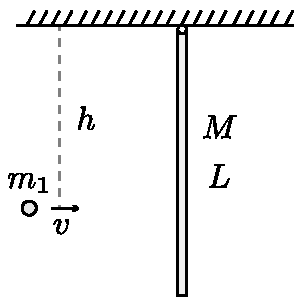
\includegraphics[width=0.22\textwidth]{2015-v2g-06-porgejoonis}
 \end{center}
 %\vspace{-30pt}
\end{wrapfigure}

Algselt paigal olev rippuv varras massiga $M$ ning pikkusega $L$ on fikseeritud ülemisest otsast vabalt pöörleva kinnitusega. Varda inertsimoment otspunkti suhtes on $I=\frac{1}{3}ML^2$. Teraspall massiga $m_1$ lendab vastu varrast ning tabab seda kaugusel $h$ riputuspunktist. Põrge on elastne, st soojuskadudeta. Huvitaval kombel jääb teraskuul pärast põrget hetkeks paigale ning hakkab seejärel vertikaalselt alla langema. Leidke kauguse $h$ väärtus, mille korral niisugune seismajäämine võimalik on.

\hint
Kuna põrge on elastne, säilib põrke käigus kineetiline energia. Impulsi kohta sama aga ei saa öelda, sest põrke ajal mõjuvad kinnituspunktile jõud. Küll aga säilib süsteemis summaarne impulsimoment kinnituspunkti suhtes, sest põrke ajal on kinnituspunktile mõjuvate jõudude õlad nullid ning põrge toimub nii kiiresti, et raskusjõuga pole vaja arvestada.

\solu
Elastse põrke korral säilib kineetiline energia. Teisalt ei saa me aga rääkida impulsi jäävusest, sest põrke ajal mõjuvad ka kinnituspunktis suured jõud. Küll aga säilib süsteemi summaarne impulsimoment kinnituspunkti suhtes, sest põrke ajal kinnituspunktis mõjuvate jõudude õlad on siis nullid ning põrge toimub nii kiiresti, et raskusjõuga pole vaja arvestada.

Paneme esmalt kirja energia jäävuse seaduse. Algselt on kuulil kineetiline energia $E_k=m_1v^2/2$. Pärast põrget on vardal kineetiline energia $E_v=I\omega^2/2$, kus $\omega$ on lati pöörlemise nurkkiirus. Niisiis,
\[
\frac{m_1v^2}{2}=\frac{I\omega^2}{2}.
\]

Asume nüüd impulsimomendi seadust avaldama. Enne põrget on liikuva kuuli impulsimoment kinnituspunkti suhtes $L_k=m_1vh$ ning vahetult pärast põrget on pöörleva varda impulsimoment $L_v=I\omega$. Niisiis,
\[
m_1vh=I\omega.
\]

Nüüd on jäänud veel lahendada neist kahest võrrandist koosnev süsteem ning avaldada otsitav kõrgus $h$. Võib lahendada asendusvõttega, aga võime ka näiteks võtta teise võrrandi mõlemad pooled ruutu ning jagada läbi esimese võrrandiga, saades
\[
m_1h^2 = I,\quad \text{millest} \quad h = \sqrt{\frac{I}{m_1}}=\sqrt{\frac{M}{3m_1}}L.
\]

\probeng{Collision}
\begin{wrapfigure}{l}{0.22\textwidth}
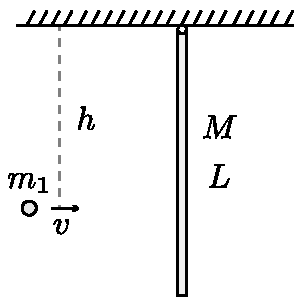
\includegraphics[width=0.22\textwidth]{2015-v2g-06-porgejoonis}
\end{wrapfigure}
An initially resting rod of mass $M$ and length $L$ is hanging from the ceiling so that its upper tip is fixed with a freely rotating attachment. The rod’s moment of inertia with respect to the tip is $I=\frac{1}{3}ML^2$. A steel ball with a mass $m_1$ flies against the rod and hits it at a distance $h$ from the fixed tip. The collision is elastic, which means there is no heat loss. Interestingly, the ball stays put for a moment after the collision and then starts to fall down vertically. Find the value of $h$ so that such a moment of stillness is possible.

\hinteng
Because the collision is elastic the kinetic energy will be preserved during the collision. You cannot say the same for momentum because forces are applied to the attachment points during the collision. However, the total angular momentum with respect to the attachment point is preserved in the system because during the collision the torque arms applied to the attachment point are zero and the collision happens so fast that you do not have to consider the gravity force.

\solueng
Kinetic energy is preserved during an elastic collision. On the other hand we are not dealing with conservation of momentum because during the collision big forces are applied to the attachment as well. However, the total angular momentum is preserved with respect to the attachment point because during the collision the force arms applied to the attachment point are then zero and the collision happens so fast that you can neglect gravity force.\\
Let us write down the conservation of energy. Initially the ball has kinetic energy $E_k=m_1v^2/2$. After the collision the rod has kinetic energy $E_v=I\omega^2/2$ where $\omega$ is the angular velocity of the rod’s rotation. So,
\[
\frac{m_1v^2}{2}=\frac{I\omega^2}{2}.
\] 
Let us now start to express the conservation of angular momentum. Before the collision the moving ball has angular momentum $L_k=m_1vh$ with respect to the attachment point and momentarily after the collision the rotating rod has the angular momentum $L_v=I\omega$. So,
\[
m_1vh=I\omega.
\]
Now we have to solve the system of these two equations and express the desired height $h$. This can be solved with replacement but we can also square both of the sides of the second equation and divide them by the first equation, getting
\[
m_1h^2 = I,\quad \text{from which} \quad h = \sqrt{\frac{I}{m_1}}=\sqrt{\frac{M}{3m_1}}L.
\]
\probend